\documentclass[9pt,aspectratio=169]{beamer}
\usepackage[T1]{fontenc}
\usepackage[utf8]{inputenc}
\usepackage{lmodern}
\usepackage{graphicx}
\usepackage{booktabs}
\usepackage{array}
\usepackage{xcolor}
\usepackage{ragged2e}
\usepackage{appendixnumberbeamer}

\definecolor{navy}{HTML}{1F3A5F}
\definecolor{teal}{HTML}{2A9D8F}
\definecolor{orange}{HTML}{E76F51}
\definecolor{gold}{HTML}{E9C46A}
\definecolor{grey}{HTML}{8D99AE}

\usetheme{default}
\usecolortheme{default}
\setbeamercolor{palette primary}{bg=navy,fg=white}
\setbeamercolor{palette secondary}{bg=navy,fg=white}
\setbeamercolor{palette tertiary}{bg=navy,fg=white}
\setbeamercolor{title}{fg=navy}
\setbeamercolor{frametitle}{bg=navy,fg=white}
\setbeamercolor{structure}{fg=navy}
\setbeamercolor{block title}{bg=teal,fg=white}
\setbeamercolor{block body}{bg=teal!8}
\setbeamercolor{section in toc}{fg=navy}
\setbeamertemplate{navigation symbols}{}
\setbeamertemplate{footline}[frame number]
\setbeamerfont{frametitle}{series=\bfseries}
\setbeamertemplate{itemize items}[circle]
\setbeamertemplate{itemize subitem}[triangle]

\newcommand{\good}{\textcolor{teal}{\textbf{Selected}}}
\newcommand{\bad}{\textcolor{grey}{rejected}}

\title{\textbf{Counterparty Credit Risk Engine}}
\subtitle{Final Presentation: Methods, Trade-offs, and Results}
\author{Berkeley MFE Industry Project -- Capitolis}
\date{\today}

\begin{document}

\begin{frame}
  \titlepage
\end{frame}

\begin{frame}{Agenda}
  \tableofcontents
\end{frame}

% ================================================================ SECTION 0
\section{Project at a Glance}

\begin{frame}{The book, and what we built}
  \begin{columns}[T]
    \begin{column}{0.55\textwidth}
      \textbf{16 trades, 3 counterparties}
      \begin{itemize}
        \item 8 equity total-return swaps
        \item 4 bond forwards, 4 bond total-return swaps
        \item 37 equities (US + Tokyo) + USDJPY
      \end{itemize}
      \vspace{6pt}
      \textbf{A full Monte Carlo engine, built from scratch}
      \begin{itemize}
        \item Joint stochastic simulation of every risk factor
        \item Exposure, Greeks, stress, CVA/DVA/FVA/KVA, SA-CVA, SA-CCR
        \item 168 automated regression tests
      \end{itemize}
    \end{column}
    \begin{column}{0.45\textwidth}
      \textbf{Every input is real, sourced data}
      \begin{itemize}
        \item Equities/dividends: Yahoo Finance
        \item USD curve: real Databento SOFR futures
        \item Treasury yields: FRED
        \item Long end + vol cube: licensed Bloomberg data
        \item JPY curve: real JPY OIS history
      \end{itemize}
    \end{column}
  \end{columns}
\end{frame}

\begin{frame}{Exposure definition, and why two numbers}
  \[ \text{Close-out: } \max\big(V(t{+}10\text{bd}) - V(t{-}1\text{bd}),\,0\big) \qquad \text{Level: } \max(V(t),0) \]
  \begin{itemize}
    \item \textbf{Close-out} (the brief's definition, primary): the 10-day move from an already-margined start
    \item \textbf{Level} (secondary): whole mark-to-market, no margin assumed -- a no-margin upper bound
    \item Real answer sits between the two; the actual CSA's threshold/MTA/IM were not supplied
  \end{itemize}
  \vspace{6pt}
  \centering
  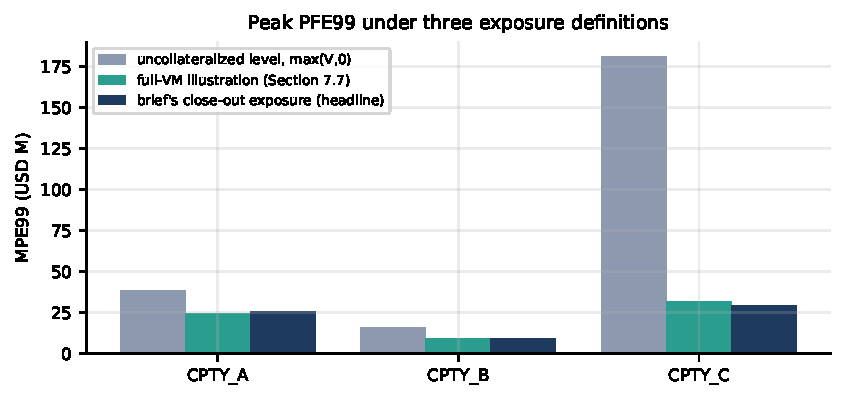
\includegraphics[width=0.55\linewidth]{figures/fig26.pdf}
\end{frame}

% ================================================================ SECTION 1
\section{Engine Architecture}

\begin{frame}{The simulation pipeline}
  \begin{enumerate}
    \item \textbf{Draw:} Latin Hypercube random numbers $\to$ correlated shocks (Cholesky)
    \item \textbf{Simulate:} step every risk factor jointly across the full time grid
    \item \textbf{Reprice:} feed simulated market states into the provided pricers, every trade, every date, every scenario
    \item \textbf{Aggregate:} net by counterparty $\to$ EE / median PFE / PFE99 / MPE
    \item \textbf{Downstream:} Greeks, stress, CVA/DVA/FVA/KVA, SA-CVA, SA-CCR -- all on the same simulated paths
  \end{enumerate}
  \vspace{8pt}
  \textbf{Risk factors simulated jointly, every scenario:}
  \begin{itemize}
    \item 37 equities + USDJPY: correlated geometric Brownian motion
    \item USD short rate: one-factor Hull-White
    \item JPY short rate: a second, independent Hull-White factor
  \end{itemize}
\end{frame}

\begin{frame}{What the simulated paths look like}
  \begin{columns}[T]
    \begin{column}{0.5\textwidth}
      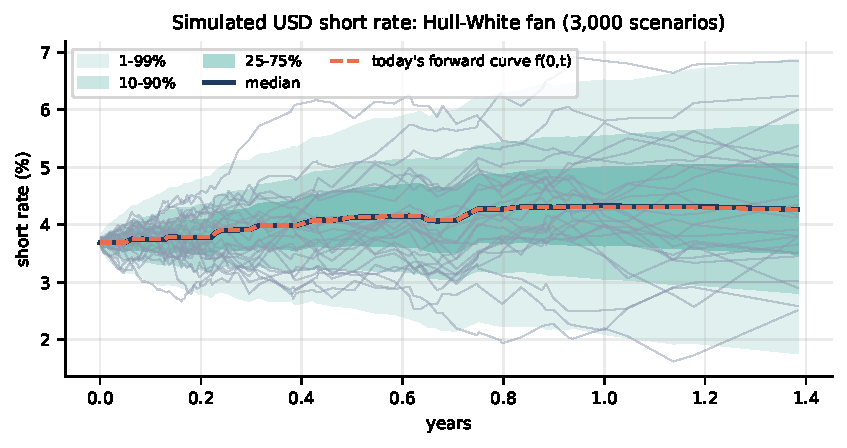
\includegraphics[width=\linewidth]{figures/fig11.pdf}
    \end{column}
    \begin{column}{0.5\textwidth}
      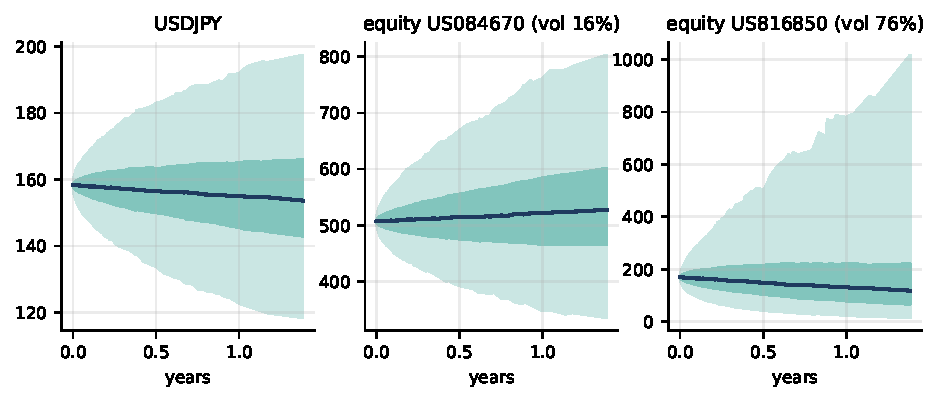
\includegraphics[width=\linewidth]{figures/fig12.pdf}
    \end{column}
  \end{columns}
  \small\centering Left: simulated USD short rate (median tracks today's forward curve, since the model is fitted to it). Right: simulated USDJPY and two equities with percentile bands.
\end{frame}

% ================================================================ SECTION 2
\section{Stochastic Model Choices}

\begin{frame}{USD rates: one-factor vs.\ two-factor Hull-White}
  \begin{columns}[T]
    \begin{column}{0.48\textwidth}
      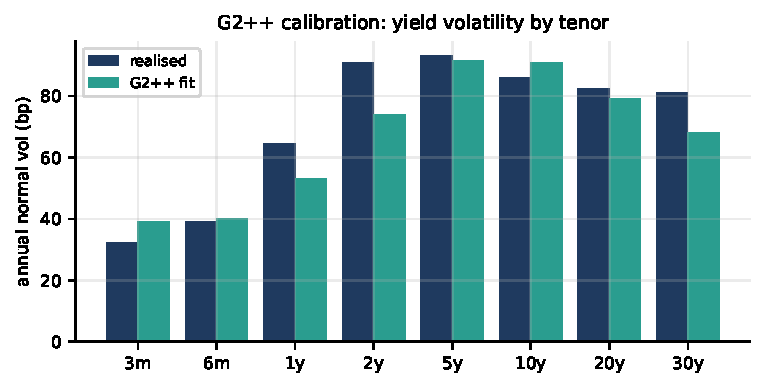
\includegraphics[width=\linewidth]{figures/fig19.pdf}
    \end{column}
    \begin{column}{0.52\textwidth}
      \small
      \begin{tabular}{p{0.44\textwidth}p{0.2\textwidth}p{0.24\textwidth}}
        \toprule
        & \textbf{1-factor} & \textbf{2-factor (G2++)} \\
        \midrule
        Fit to realised yield covariance & -- & 16.1\% error \\
        Parameter at a bound & no & $b=1.5$, $\rho{=}{-}0.95$ \\
        Effect on portfolio MPE99 & baseline & $-3\%$ \\
        \bottomrule
      \end{tabular}
      \vspace{6pt}
      \good: the two-factor fit strains to match a hump it can't represent, and moves the headline number by only 3\%. The book's rate risk is one big level bet (a single long bond), not a curve-shape bet.
    \end{column}
  \end{columns}
\end{frame}

\begin{frame}{JPY rates: a dedicated factor vs.\ a constant differential}
  \begin{columns}[T]
    \begin{column}{0.45\textwidth}
      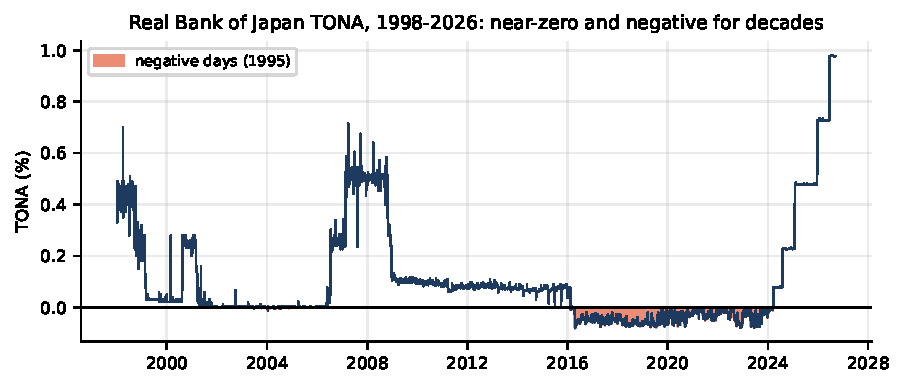
\includegraphics[width=\linewidth]{figures/fig16.pdf}
    \end{column}
    \begin{column}{0.55\textwidth}
      \small
      \textbf{Alternative rejected:} JPY names/USDJPY drift off one constant USD--JPY rate differential -- cheap, but cannot represent JPY rates moving independently, or negative.
      \vspace{4pt}
      \textbf{\good:} a second, real, simulated Hull-White factor from the JPY OIS curve.
      \begin{itemize}
        \item TONA has been negative or near-zero for most of 25 years -- a floored model can't represent this
        \item Day-to-day USD/JPY rate changes are uncorrelated ($-0.04$) despite yield \emph{levels} moving together ($\sim$0.38)
        \item Moved portfolio MPE99 attribution from \$52.1M to \$51.5M -- real, disclosed, not noise
      \end{itemize}
    \end{column}
  \end{columns}
\end{frame}

\begin{frame}{Equity/FX correlation: full matrix vs.\ PCA factor model}
  \begin{columns}[T]
    \begin{column}{0.55\textwidth}
      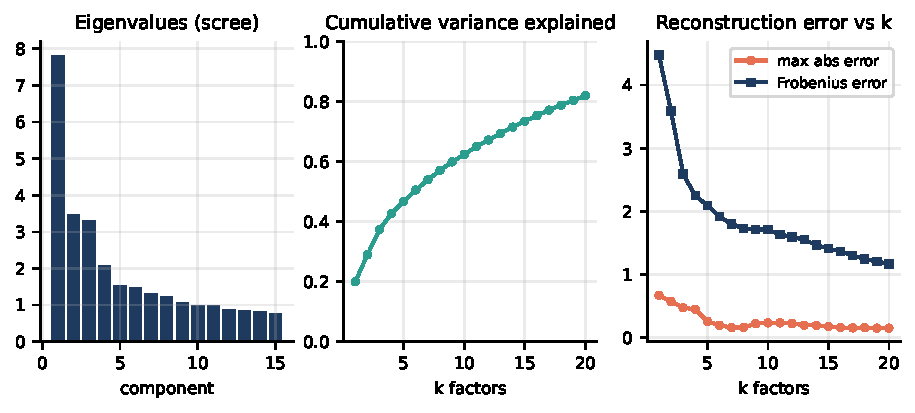
\includegraphics[width=\linewidth]{figures/fig14.pdf}
    \end{column}
    \begin{column}{0.45\textwidth}
      \small
      \begin{tabular}{p{0.32\textwidth}p{0.2\textwidth}p{0.2\textwidth}}
        \toprule
        & \textbf{Full} & \textbf{PCA k=5} \\
        \midrule
        Step time & 1.91s & 2.08s \\
        Variance explained & 100\% & 47\% \\
        \bottomrule
      \end{tabular}
      \vspace{6pt}
      \good\ full matrix: PCA is \emph{slower}, not faster, at $n{=}39$ (draws $k$ systematic + $n$ idiosyncratic, no dimensionality win). PCA kept as an explainability tool only -- factor 1 is a broad market factor, factor 2 is Japan vs.\ US.
    \end{column}
  \end{columns}
\end{frame}

\begin{frame}{Calibration: mean reversion, and implied vs.\ realised vol}
  \small
  \begin{tabular}{p{0.2\textwidth}p{0.33\textwidth}p{0.35\textwidth}}
    \toprule
    \textbf{Parameter} & \textbf{Source used} & \textbf{Why} \\
    \midrule
    Rate mean reversion ($a$) & Real USD swaption cube (implied), $a{=}0.0167$ & Standard route; decay shape is what implied vol reveals. Futures-decay cross-check gives 0.0458 (different instrument/tenor range) \\
    Rate volatility ($\sigma$) & Realised long-end Treasury vol, 0.96\% & Overnight-SOFR vol (0.63\%) understates long-end moves this book depends on; confirmed by Kupiec backtest \\
    Equity/FX volatility & Realised, 3y history & No implied-vol source available; disclosed proxy \\
    JPY mean reversion & Lowest admissible ($a{=}0.001$) & All 3 real routes (swaption, JGB, OIS) give a \emph{negative} $a$ -- JPY vol rises with tenor \\
    \bottomrule
  \end{tabular}
\end{frame}

% ================================================================ SECTION 3
\section{Simulation Methodology}

\begin{frame}{Sampling scheme: five methods compared}
  \begin{columns}[T]
    \begin{column}{0.55\textwidth}
      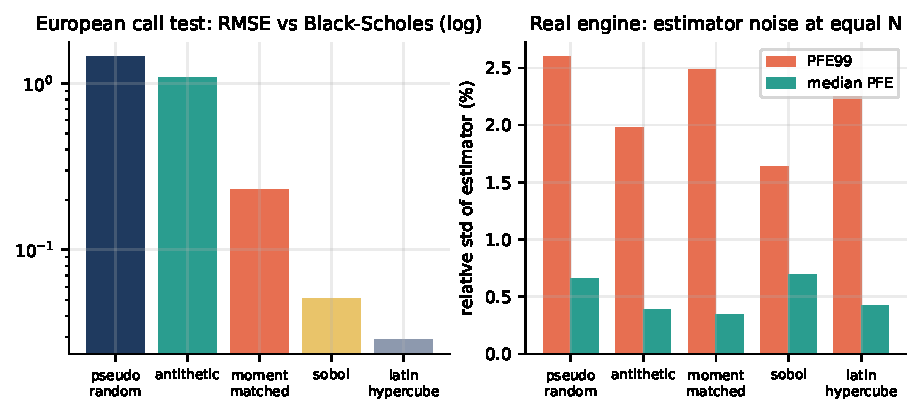
\includegraphics[width=\linewidth]{figures/fig21.pdf}
    \end{column}
    \begin{column}{0.45\textwidth}
      \small
      Tested: pseudo-random, antithetic, moment-matching, Sobol, Latin Hypercube -- on a controlled Black-Scholes benchmark and the real 663-dimensional engine.
      \vspace{6pt}
      \good\ Latin Hypercube: $\sim$51x lower error on the controlled test, and the only method better than pseudo-random on \emph{both} real-engine statistics (PFE99 and median PFE), at negligible extra cost.
    \end{column}
  \end{columns}
\end{frame}

\begin{frame}{Scenario count vs.\ precision}
  \small
  \begin{tabular}{p{0.08\textwidth}p{0.2\textwidth}p{0.18\textwidth}p{0.38\textwidth}}
    \toprule
    \textbf{$N$} & \textbf{Rel.\ SE, PFE99} & \textbf{Time (8 cores)} & \textbf{Use} \\
    \midrule
    1,000 & higher & $\sim$2 min & Iteration / what-if \\
    5,000 & moderate & $\sim$8 min & \good\ Standard reporting \\
    10,000 & lower & $\sim$15 min & Limit sign-off \\
    15,000+ & diminishing returns & -- & Not recommended \\
    \bottomrule
  \end{tabular}
  \vspace{8pt}
  Beyond $\sim$15,000 scenarios, remaining sampling error is an order of magnitude smaller than model-risk sensitivities (Section 7) -- more scenarios stop being the binding constraint on precision well before that.
\end{frame}

% ================================================================ SECTION 4
\section{Headline Results}

\begin{frame}{Headline results (5,000 scenarios, close-out exposure)}
  \begin{columns}[T]
    \begin{column}{0.4\textwidth}
      \small
      \begin{tabular}{lrr}
        \toprule
        & \textbf{MPE99} & \textbf{Peak EE} \\
        \midrule
        CPTY\_A & \$25.9M & \$4.7M \\
        CPTY\_B & \$9.6M & \$1.8M \\
        CPTY\_C & \$29.6M & \$5.2M \\
        \midrule
        \textbf{Portfolio} & \textbf{\$51.0M} & \textbf{\$11.6M} \\
        \bottomrule
      \end{tabular}
      \vspace{8pt}
      \begin{itemize}
        \item CVA \$11.7k close-out / \$247k level
        \item SA-CVA capital \$0.10M / \$2.23M
        \item SA-CCR EAD \$260M
        \item KVA (10\% CoC) \$22.4k / \$470k
      \end{itemize}
    \end{column}
    \begin{column}{0.6\textwidth}
      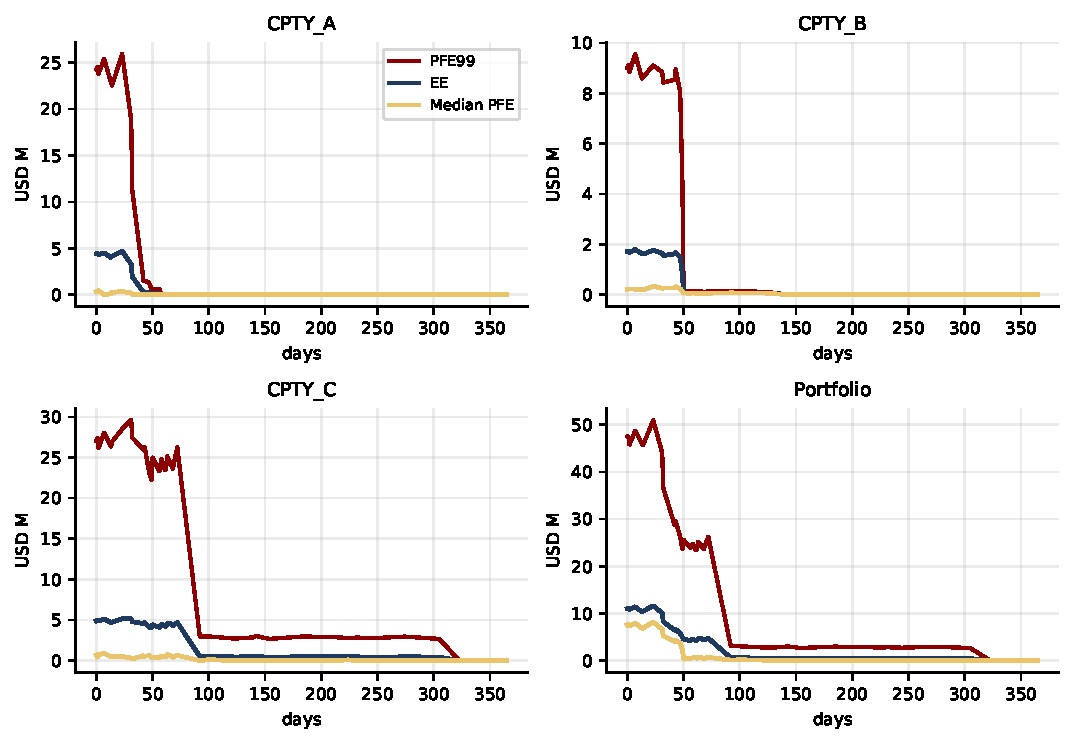
\includegraphics[width=\linewidth]{figures/fig25.pdf}
    \end{column}
  \end{columns}
\end{frame}

\begin{frame}{What drives each counterparty, and why the portfolio is close to additive}
  \begin{columns}[T]
    \begin{column}{0.55\textwidth}
      \small
      \begin{tabular}{lrr}
        \toprule
        & \textbf{Equity $\Delta$/+1\%} & \textbf{DV01/+1bp} \\
        \midrule
        CPTY\_A & -\$2.25M & \$31k \\
        CPTY\_B & -\$0.96M & -\$4k \\
        CPTY\_C & -\$1.24M & \textbf{\$594k} \\
        \bottomrule
      \end{tabular}
      \vspace{6pt}
      Rank correlation of exposures: A--B 0.34, A--C 0.33, B--C 0.12
    \end{column}
    \begin{column}{0.45\textwidth}
      \small
      \begin{itemize}
        \item A is most equity-driven; C is the rate netting set (one \$500M short forward on a 2049 Treasury)
        \item Yield-equity correlation $\approx$0.00 in our data -- no reliable offset
        \item Nothing nets \emph{across} counterparties by construction, and all three peak in the same weeks
        \item Portfolio MPE99 (\$51.0M) $\approx$ A+C (\$54.4M)
      \end{itemize}
    \end{column}
  \end{columns}
\end{frame}

% ================================================================ SECTION 5
\section{Sensitivities (Greeks)}

\begin{frame}{Method, and the cost of a naive approach}
  \begin{columns}[T]
    \begin{column}{0.45\textwidth}
      \small
      \begin{itemize}
        \item Bump-and-reprice with \textbf{common random numbers}: same draws base/bumped $\to$ noise \$245k $\to$ \$1k (\textbf{282x lower})
        \item Equity/FX bumps rescale simulated GBM paths exactly -- no resimulation
        \item Rate/vol bumps need a genuine resimulation
      \end{itemize}
    \end{column}
    \begin{column}{0.55\textwidth}
      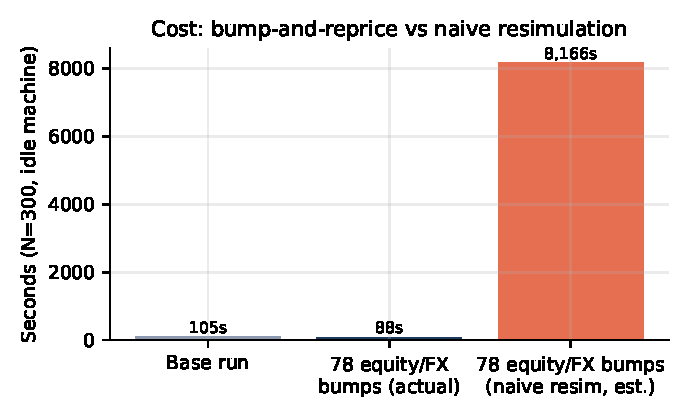
\includegraphics[width=\linewidth]{figures/fig_greeks_cost.pdf}
    \end{column}
  \end{columns}
\end{frame}

\begin{frame}{Bump-and-reprice vs.\ pathwise vs.\ adjoint}
  \small
  \begin{tabular}{p{0.22\textwidth}p{0.22\textwidth}p{0.42\textwidth}}
    \toprule
    \textbf{Method} & \textbf{Cost} & \textbf{Verdict} \\
    \midrule
    Bump, independent draws & baseline, very noisy & \bad: noise swamps the signal \\
    Bump, common random numbers & $\sim$260s (equity EE) & \good: works on black-box pricers, works for quantiles \\
    Pathwise (closed form) & 0.2--0.4s & \good\ for equity/FX only: $\sim$1000x faster, validated to median 0.02\%/worst 0.4\% vs.\ bump-and-reprice \\
    Adjoint differentiation & would price all Greeks for $\sim$3-5 valuations & \bad: needs pricers rewritten in differentiable form -- out of scope \\
    \bottomrule
  \end{tabular}
\end{frame}

\begin{frame}{Rate DV01: zero-grid bump vs.\ par-instrument Jacobian}
  \begin{columns}[T]
    \begin{column}{0.5\textwidth}
      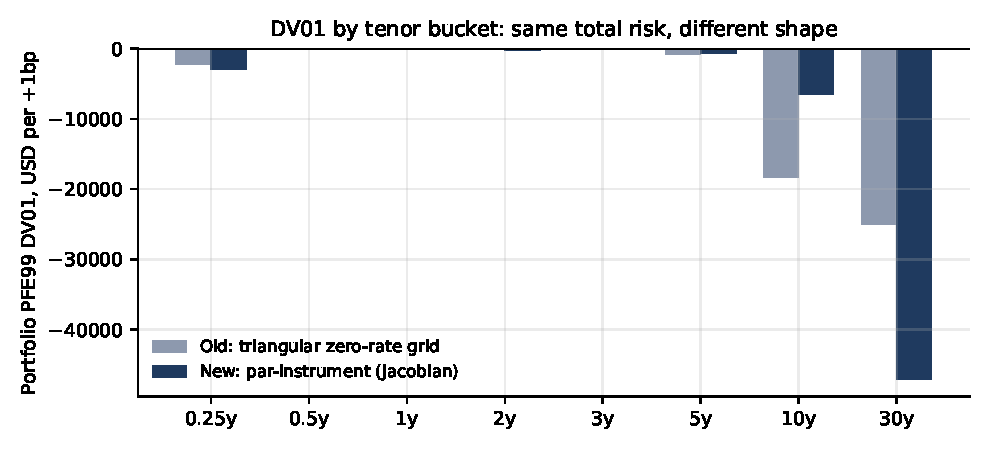
\includegraphics[width=\linewidth]{figures/fig_dv01_compare.pdf}
    \end{column}
    \begin{column}{0.5\textwidth}
      \small
      \textbf{Old:} bump the \emph{fitted} zero curve at 8 hand-picked tenors, triangular interpolation.

      \textbf{\good\ New:} bump the curve's own $\sim$45 native construction pillars (real SOFR futures + Bloomberg points), grouped into the same 8 buckets -- the genuine par-instrument (Jacobian) sensitivity.
      \vspace{4pt}
      \begin{itemize}
        \item 30y bucket: \textbf{82\%} of DV01 (new) vs.\ 54\% (old)
        \item Old grid smeared the 20--50y risk, where the 2049 bond forward lives, into the 10y bucket
        \item Both sum to the independent parallel bump within 0.1\%
      \end{itemize}
    \end{column}
  \end{columns}
\end{frame}

\begin{frame}{An exact rate Greek, reusing the same simulated draws}
  \small
  In one-factor Hull-White, $r(t)=x(t)+\alpha(t)$: $x(t)$ is the simulated random factor; $\alpha(t)$ is deterministic, depends only on the curve. A curve bump (fixed $a,\sigma$) leaves $x(t)$ \textbf{identical} to the base run.
  \begin{itemize}
    \item The whole bump effect is one closed-form number per date, added to the base run's own paths
    \item \textbf{No resimulation. No new random draws.}
    \item Validated against a true independent resimulation: agreement to $\mathbf{10^{-15}}$ relative precision
  \end{itemize}
  \vspace{6pt}
  \textbf{Separately: does Latin Hypercube itself reduce Greeks noise?} Tested directly -- mixed result:
  \centering
  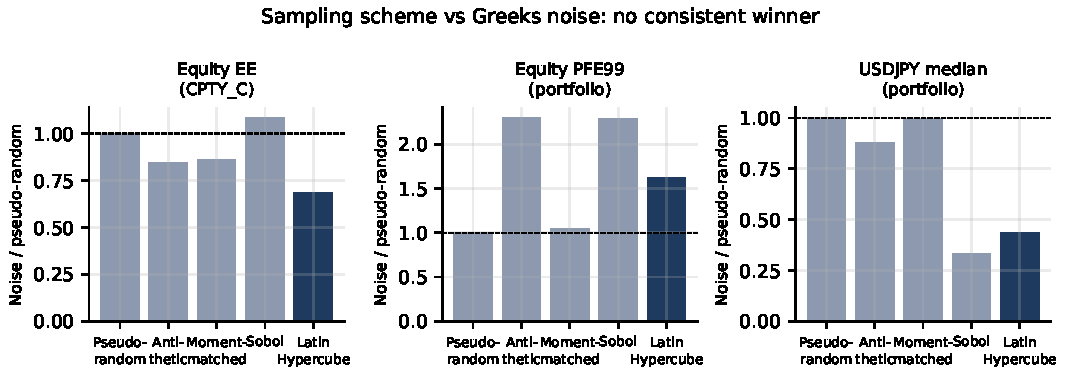
\includegraphics[width=0.55\linewidth]{figures/fig_sampling_greeks.pdf}
\end{frame}

% ================================================================ SECTION 6
\section{Stress Testing}

\begin{frame}{Design: 13 fixed scenarios, same random draws as base}
  \begin{columns}[T]
    \begin{column}{0.5\textwidth}
      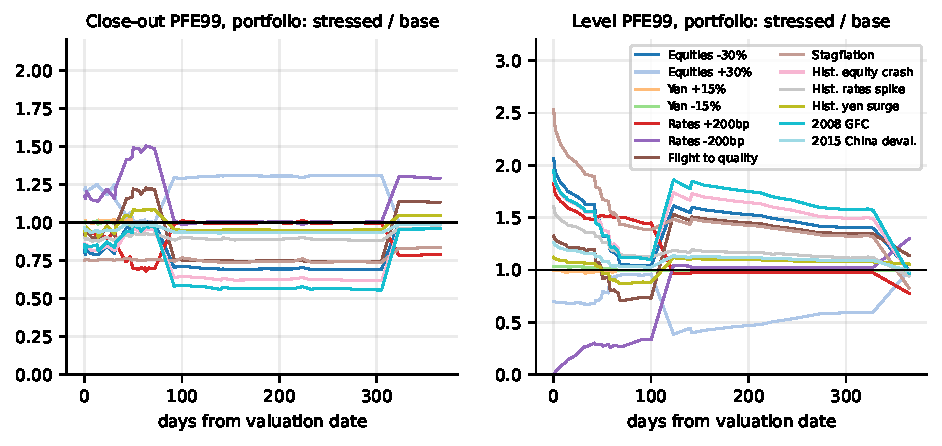
\includegraphics[width=\linewidth]{figures/fig33.pdf}
    \end{column}
    \begin{column}{0.5\textwidth}
      \small
      \begin{itemize}
        \item 8 hypothetical: equities $\pm$30\%, yen $\pm$15\%, rates $\pm$200bp, flight-to-quality, stagflation
        \item 5 historical replays, chosen by an objective worst-window rule, not by hand
        \item Read at every date, every trade, every counterparty
      \end{itemize}
      \vspace{6pt}
      Close-out MPE99 moves at most $-24\%$ to $+23\%$; level moves up to $+89\%$ -- margin is why. Equity swaps react only to equity/FX; bond trades react only to rates.
    \end{column}
  \end{columns}
\end{frame}

\begin{frame}{Extending the history: 2008 and 2015}
  \begin{columns}[T]
    \begin{column}{0.5\textwidth}
      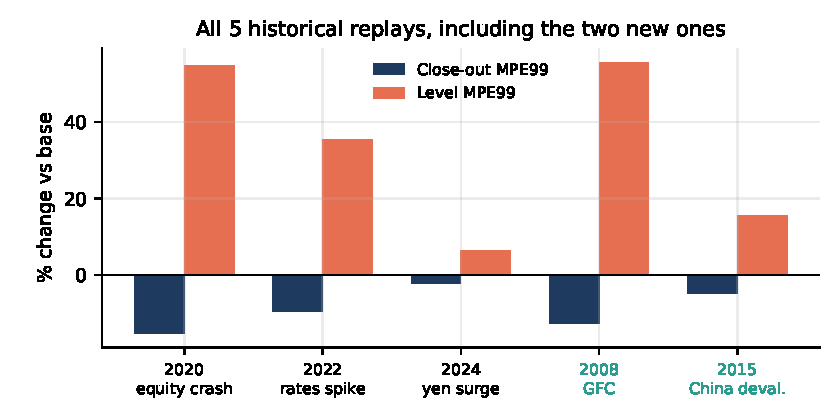
\includegraphics[width=\linewidth]{figures/fig_hist_scenarios.pdf}
    \end{column}
    \begin{column}{0.5\textwidth}
      \small
      Extended public price history back to 2007 (28 of 37 names covered), found the worst 10-day window inside two named crises:
      \begin{itemize}
        \item \textbf{2008 GFC:} Sep 29 -- Oct 10, 2008; $-23\%$ median / $-44\%$ worst single-name
        \item \textbf{2015 China deval.:} Aug 2015, $-6.8\%$ median
      \end{itemize}
      \vspace{6pt}
      \textbf{Result:} both land \emph{inside} the range the existing scenarios already covered -- a validation finding, not just more coverage.
    \end{column}
  \end{columns}
\end{frame}

% ================================================================ SECTION 7
\section{Model Validation and Model Risk}

\begin{frame}{Four independent validation checks}
  \small
  \begin{tabular}{p{0.19\textwidth}p{0.28\textwidth}p{0.4\textwidth}}
    \toprule
    \textbf{Check} & \textbf{Method} & \textbf{Result} \\
    \midrule
    Martingale test & Discounted paths average to today's price & Pass \\
    Parametric VaR benchmark & Delta-normal VaR vs.\ full MC P\&L & \$11.4M vs.\ \$11.7M (ratio 0.98) \\
    Kupiec backtest (99\%) & Historical exceedances vs.\ prediction & 4/6/2 exceptions vs.\ 2.4 expected -- all pass \\
    Excel parametric checks & Independent spreadsheet formulas, public data & 0.1--7\% agreement across 4 checks \\
    \bottomrule
  \end{tabular}
  \vspace{10pt}
  The Excel workbook recomputes calibrated vols live (\texttt{=STDEV(LN(Pt/Pt-1))*SQRT(252)}), the simulated vol against the closed-form $\text{vol}\times\sqrt{T}$, and a Monte Carlo vega against the closed-form Black vega under a $\pm1\%$ bump -- every number a live formula on public data, no code trust required.
\end{frame}

\begin{frame}{Model risk: what actually moves the headline number}
  \small
  \begin{tabular}{lr}
    \toprule
    \textbf{Perturbation (base portfolio MPE99 = \$51.5M)} & \textbf{Change} \\
    \midrule
    Equity/FX vol $\times2$ & $+71\%$ \\
    Equity correlations, 30\% toward 1 & $+22\%$ \\
    Equity/FX vol $\times1.25$ & $+19\%$ \\
    Rate--equity dependence, both fall together & $+18\%$ \\
    Rate volatility $\times1.25$ & $+9\%$ \\
    Rate--equity dependence, offsetting & $-15\%$ \\
    Mean reversion $a\times3$ & $-5\%$ \\
    Two-factor rate model (G2++) instead of one-factor & $-3\%$ \\
    \bottomrule
  \end{tabular}
  \vspace{8pt}
  \textbf{Conclusion:} equity volatility, correlation, and the data-unresolvable rate-equity dependence dominate. The one- vs.\ two-factor rate-model choice explored in depth is, by comparison, one of the \emph{smallest} levers -- the strongest argument for the simpler model.
\end{frame}

% ================================================================ SECTION 8
\section{Credit and Capital: xVA}

\begin{frame}{CVA: methodology and results}
  \begin{columns}[T]
    \begin{column}{0.5\textwidth}
      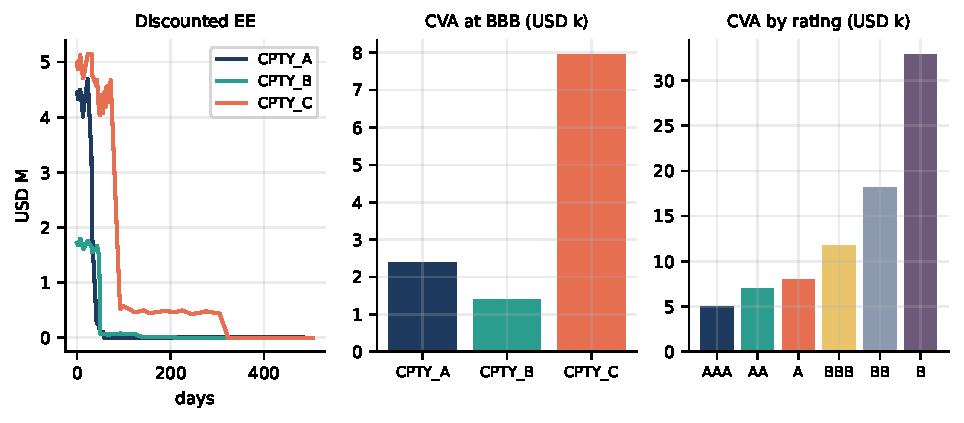
\includegraphics[width=\linewidth]{figures/fig36.pdf}
    \end{column}
    \begin{column}{0.5\textwidth}
      \small
      \begin{itemize}
        \item No CDS available $\to$ ICE BofA bond-index OAS proxy by rating (Basel MAR50.32(3)-compliant)
        \item Credit-triangle hazard-rate survival model: $\text{hazard} \approx \text{spread}/(1{-}\text{recovery})$
        \item LGD 60\%; all three counterparties proxied at BBB
      \end{itemize}
      \vspace{6pt}
      \textbf{Value delivered:} the sensitivity chain -- CVA01, the rating table (AAA \$5.0k $\to$ B \$32.8k), SA-CVA weighted sensitivities by risk class -- matters more than the point-in-time number itself.
    \end{column}
  \end{columns}
\end{frame}

\begin{frame}{DVA, FVA, and KVA (extra credit)}
  \begin{columns}[T]
    \begin{column}{0.45\textwidth}
      \small
      \begin{tabular}{lrr}
        \toprule
        & \textbf{Close-out} & \textbf{Level} \\
        \midrule
        CVA & \$11.7k & \$247k \\
        DVA & \$11.2k & \$7.5k \\
        FVA & \$0.5k & \$240.0k \\
        KVA (10\% CoC) & \$22.4k & \$470k \\
        \bottomrule
      \end{tabular}
    \end{column}
    \begin{column}{0.55\textwidth}
      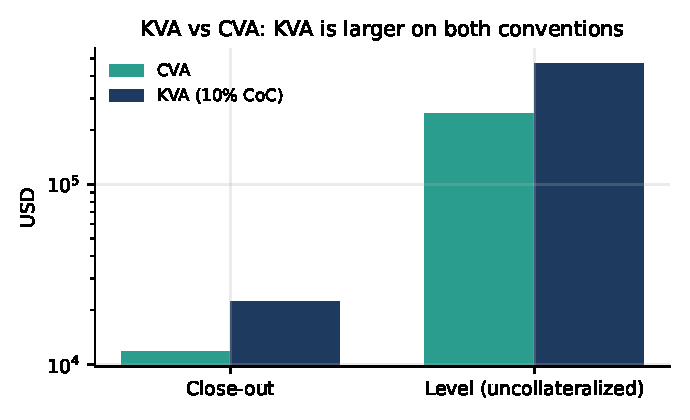
\includegraphics[width=\linewidth]{figures/fig_kva_compare.pdf}
    \end{column}
  \end{columns}
  \small\vspace{4pt}
  KVA: $K(t)=8\%\times\text{RW}\times\alpha\times\text{EPE}(t)$, cost-of-capital swept 8/10/12\% (none given). Exceeds CVA because it scales the whole EPE profile by a fixed ratio, not a small IG default probability -- explicitly illustrative.
\end{frame}

\begin{frame}{Regulatory capital: SA-CVA and SA-CCR}
  \begin{columns}[T]
    \begin{column}{0.55\textwidth}
      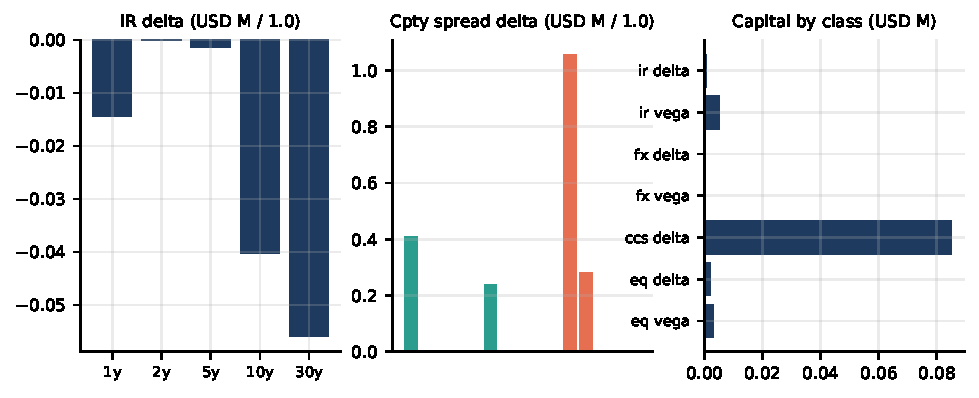
\includegraphics[width=\linewidth]{figures/fig37.pdf}
    \end{column}
    \begin{column}{0.45\textwidth}
      \small
      \begin{itemize}
        \item SA-CVA capital: \$0.10M close-out / \$2.23M level (RWA \$1.2M / \$27.8M)
        \item Dominated by counterparty credit-spread risk in both conventions
        \item SA-CCR exposure at default: \$260M, dominated by the replacement cost of BF\_0003
      \end{itemize}
    \end{column}
  \end{columns}
\end{frame}

\begin{frame}{Extra credit: a risky-bond sample trade}
  \small
  The kickoff brief flagged \emph{``Risk bonds + CDS data for new sample trades''}. Delivered:
  \begin{itemize}
    \item A sample risky-bond forward (25M notional, 5\% BBB corporate; not part of the ESF book)
    \item Priced and simulated with a real issuer credit curve, re-anchored at every simulated node
    \item Same hazard-rate survival model and bond-index proxy construction as the counterparty CVA
  \end{itemize}
  \vspace{6pt}
  \textbf{Limitation, disclosed:} no real CDS quotes were obtainable for a hypothetical issuer, so the issuer curve is a bond-index proxy, not actual CDS -- delivered in spirit, not the full ask.
\end{frame}

% ================================================================ SECTION 9
\section{Conclusions}

\begin{frame}{Recap: every trade-off, one line each}
  \scriptsize
  \begin{tabular}{p{0.3\textwidth}p{0.62\textwidth}}
    \toprule
    \textbf{Decision} & \textbf{Why} \\
    \midrule
    One-factor Hull-White, not two-factor & Two-factor moves MPE99 by only $-3\%$; 16\% fit error; book is a level bet \\
    Dedicated JPY Hull-White factor & Real, independent JPY rate risk incl.\ negative rates; moved MPE99 \$52.1M$\to$\$51.5M \\
    Full correlation matrix, not PCA & PCA is slower at $n{=}39$, no accuracy gain; kept as explainability tool only \\
    Latin Hypercube sampling & Best of 5 schemes on controlled \& real-engine tests; no consistent Greeks-noise edge \\
    Close-out exposure primary, level secondary & The brief's definition; level is an honest no-margin upper bound \\
    Bump-and-reprice with CRN, pathwise cross-check & 282x noise reduction; pathwise 1000x faster for linear risk \\
    Par-instrument DV01 buckets & Corrected real mis-attribution: 82\% vs.\ 54\% of risk in the 30y bucket \\
    Exact LHS-reuse rate Greek & Eliminates resimulation cost for curve-only bumps, $10^{-15}$ validated \\
    Rating-proxy CVA/DVA/FVA/KVA & No CDS/real ratings available; Basel-compliant proxy, fully disclosed \\
    \bottomrule
  \end{tabular}
\end{frame}

\begin{frame}{Recommendations for production}
  \begin{itemize}
    \item Keep the one-factor Hull-White rate model; revisit only if curve-shape risk grows materially
    \item Keep the full correlation matrix; retain PCA as an explainability exhibit
    \item Keep Latin Hypercube as the default sampling scheme
    \item Adopt the par-instrument DV01 buckets as the primary rate-risk breakdown
    \item Treat CVA/DVA/FVA/KVA as sensitivity-generating tools first, point estimates second
  \end{itemize}
  \vspace{10pt}
  \textbf{Open items for the next phase:} real counterparty ratings or CDS, Capitolis' own credit/funding spread, a real capital methodology and cost of capital for KVA, a decision on wrong-way risk, and the true CSA terms (threshold, MTA, IM).
\end{frame}

\begin{frame}
  \centering
  \vspace{2cm}
  {\Huge \textcolor{navy}{\textbf{Thank you}}}\\[8pt]
  {\large Questions and discussion}
\end{frame}

% ================================================================ APPENDIX
\appendix
\begin{frame}
  \centering
  \vspace{2cm}
  {\Huge \textcolor{navy}{\textbf{Appendix}}}\\[8pt]
  {\large Backup detail}
\end{frame}

\begin{frame}{Appendix: correction attribution, one at a time}
  \small
  \begin{tabular}{p{0.78\textwidth}p{0.14\textwidth}}
    \toprule
    \textbf{Step} & \textbf{Portfolio MPE99} \\
    \midrule
    Earlier version (flat curve beyond 6.5y, SOFR-overnight $\sigma$, no JPY factor, USDJPY drift sign error) & \$45.7M \\
    + Corrected USDJPY drift sign & \$47.8M \\
    + Long-end volatility fit and 10y-yield correlations & \$52.7M \\
    + Bloomberg long end spliced onto the USD curve & \$52.1M \\
    + JPY Hull-White factor (final model) & \$51.5M \\
    \bottomrule
  \end{tabular}
\end{frame}

\begin{frame}{Appendix: JPY mean-reversion calibration routes}
  \small
  All three real-data routes for JPY give a negative $a$ (vol rises with tenor, the reverse of what Hull-White assumes), so the Ho-Lee lower bound ($a{=}0.001$) is used instead of an invalid fit.
  \centering
  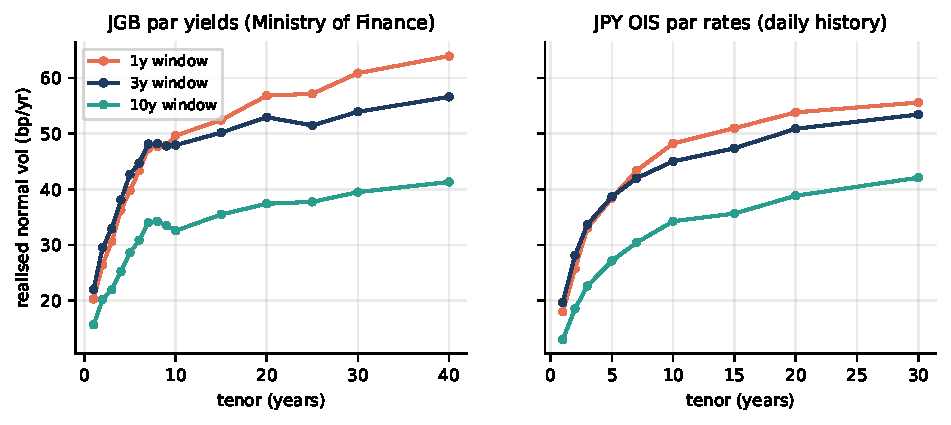
\includegraphics[width=0.6\linewidth]{figures/fig24.pdf}
\end{frame}

\begin{frame}{Appendix: negative-rate capability, synthetic demonstration}
  \small
  Our only real JPY curve snapshot (Aug 2026) is positive after BOJ hikes, so the negative case is demonstrated synthetically: Hull-White started from a synthetic $-0.10\%$ flat curve.
  \centering
  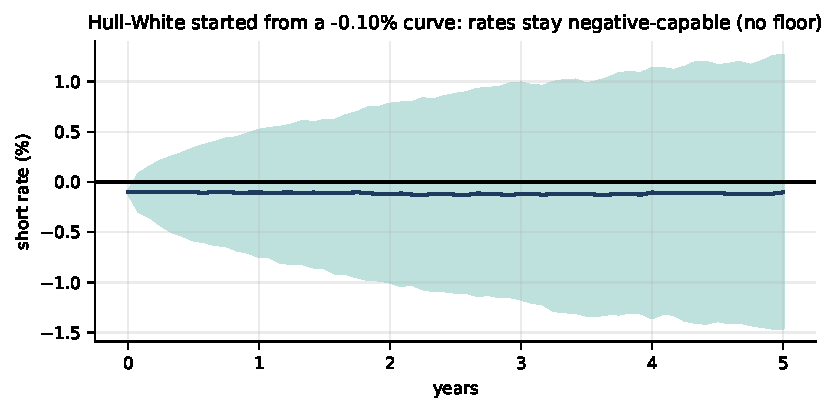
\includegraphics[width=0.55\linewidth]{figures/fig17.pdf}
\end{frame}

\begin{frame}{Appendix: exposure diagnostics}
  \begin{columns}[T]
    \begin{column}{0.5\textwidth}
      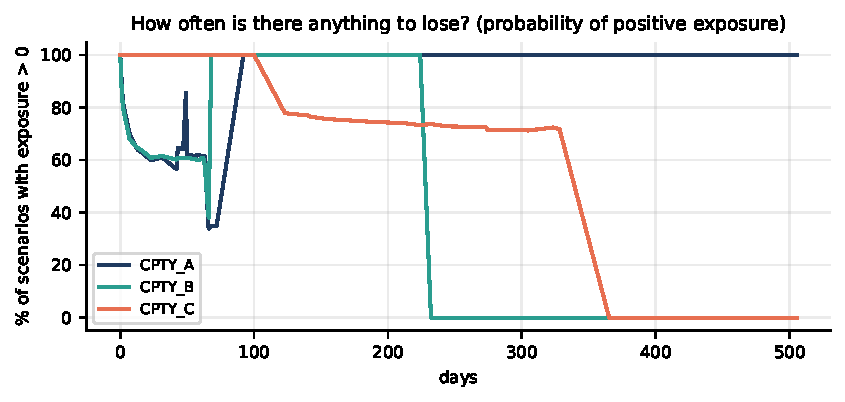
\includegraphics[width=\linewidth]{figures/fig28.pdf}
    \end{column}
    \begin{column}{0.5\textwidth}
      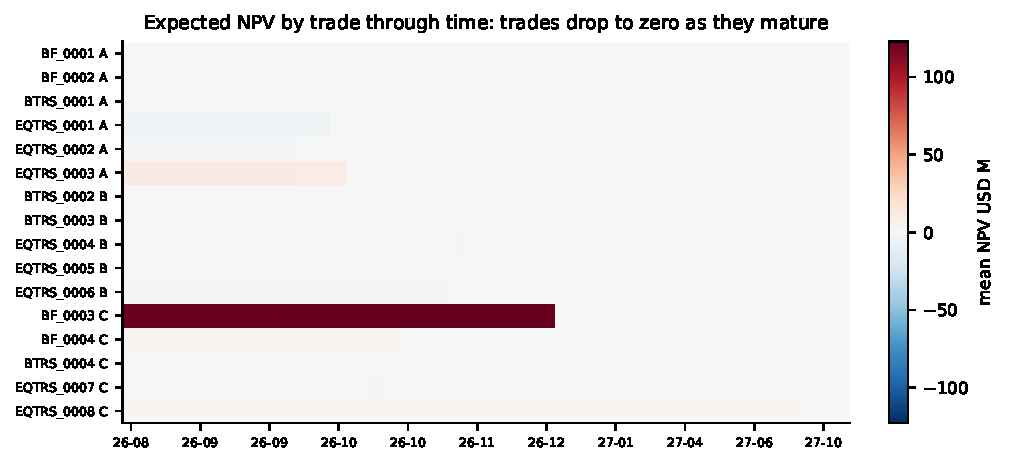
\includegraphics[width=\linewidth]{figures/fig30.pdf}
    \end{column}
  \end{columns}
  \small\centering Left: probability of positive exposure by counterparty. Right: expected NPV by trade -- BF\_0003 dominates and disappears at its Dec 2026 settlement.
\end{frame}

\begin{frame}{Appendix: full-VM comparison and PCA exposure cross-check}
  \begin{columns}[T]
    \begin{column}{0.5\textwidth}
      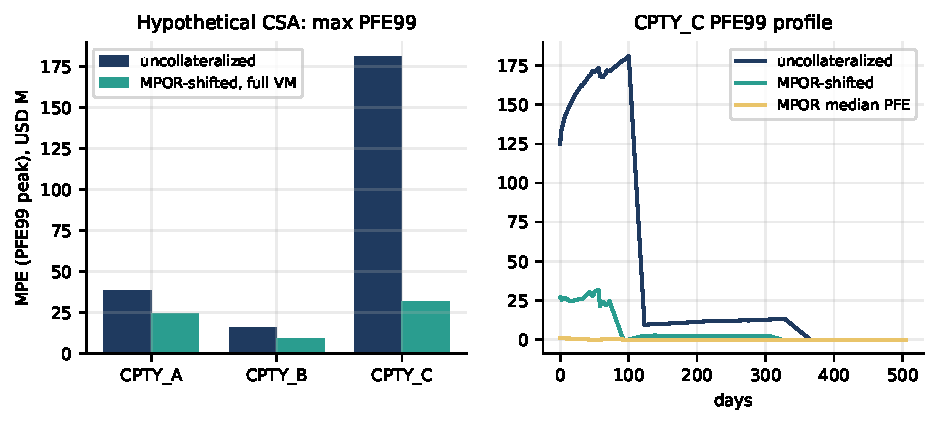
\includegraphics[width=\linewidth]{figures/fig31.pdf}
    \end{column}
    \begin{column}{0.5\textwidth}
      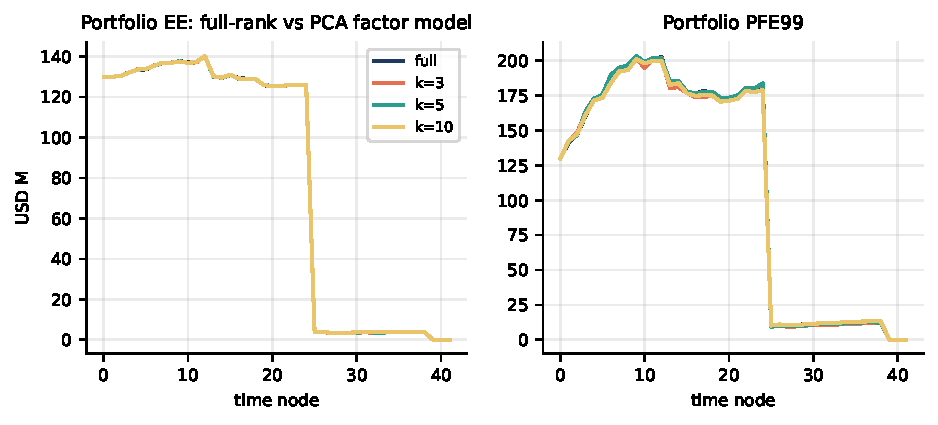
\includegraphics[width=\linewidth]{figures/fig32.pdf}
    \end{column}
  \end{columns}
  \small\centering Left: peak PFE99 under a hypothetical full-VM CSA. Right: level exposure under the full correlation matrix vs.\ a $k$-factor PCA model -- curves coincide closely from $k{=}5$.
\end{frame}

\begin{frame}{Appendix: per-trade stress sensitivity heat map}
  \centering
  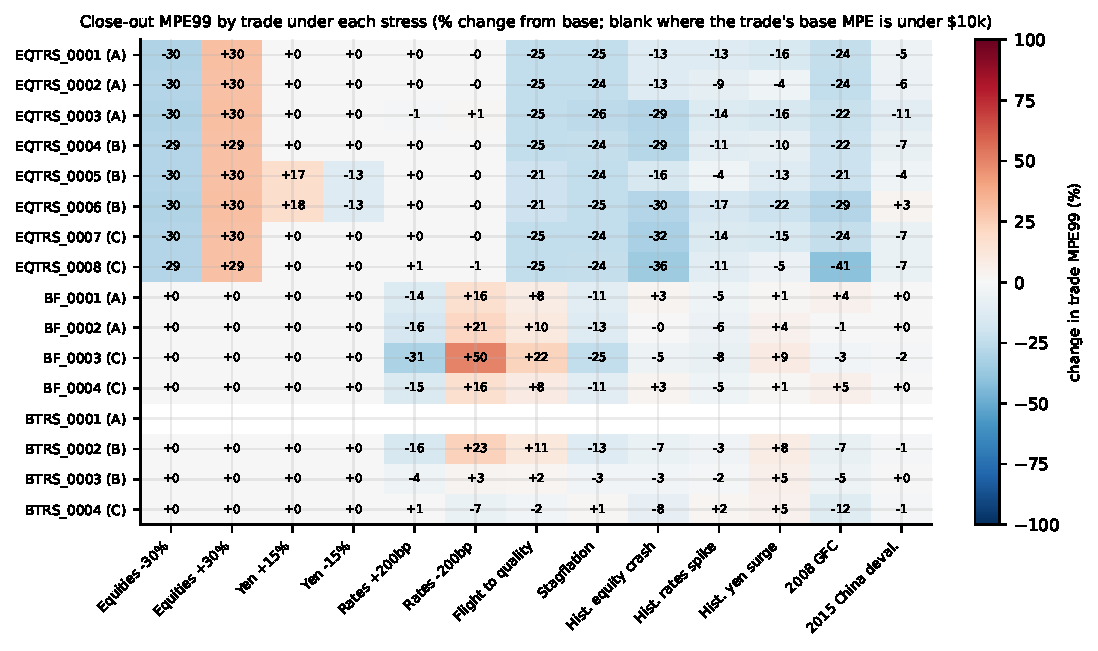
\includegraphics[width=0.85\linewidth]{figures/fig34.pdf}
\end{frame}

\begin{frame}{Appendix: xVA components and discounted exposure}
  \begin{columns}[T]
    \begin{column}{0.5\textwidth}
      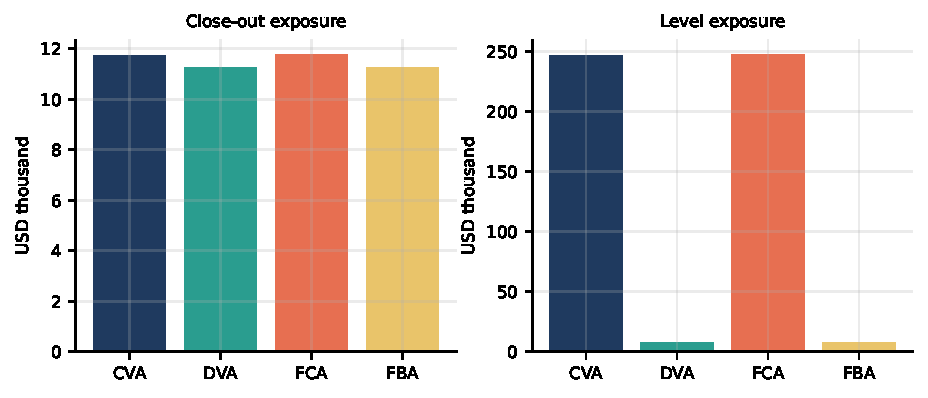
\includegraphics[width=\linewidth]{figures/fig38.pdf}
    \end{column}
    \begin{column}{0.5\textwidth}
      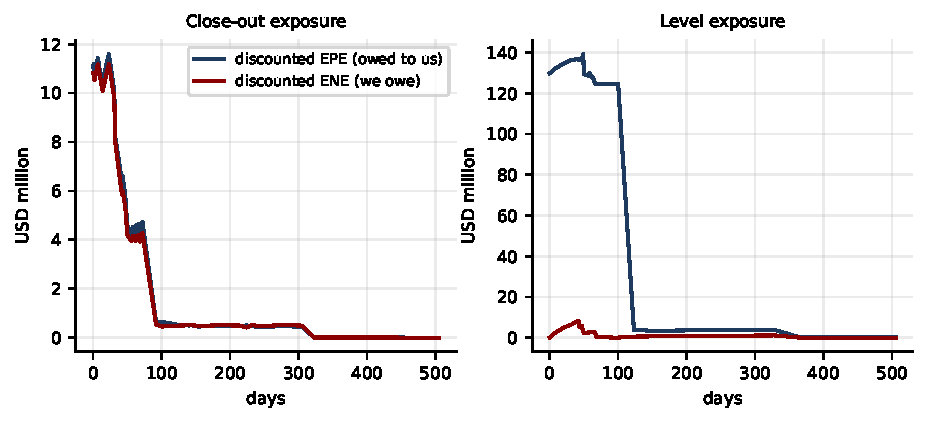
\includegraphics[width=\linewidth]{figures/fig39.pdf}
    \end{column}
  \end{columns}
\end{frame}

\begin{frame}{Appendix: correlation matrix and factor loadings}
  \begin{columns}[T]
    \begin{column}{0.5\textwidth}
      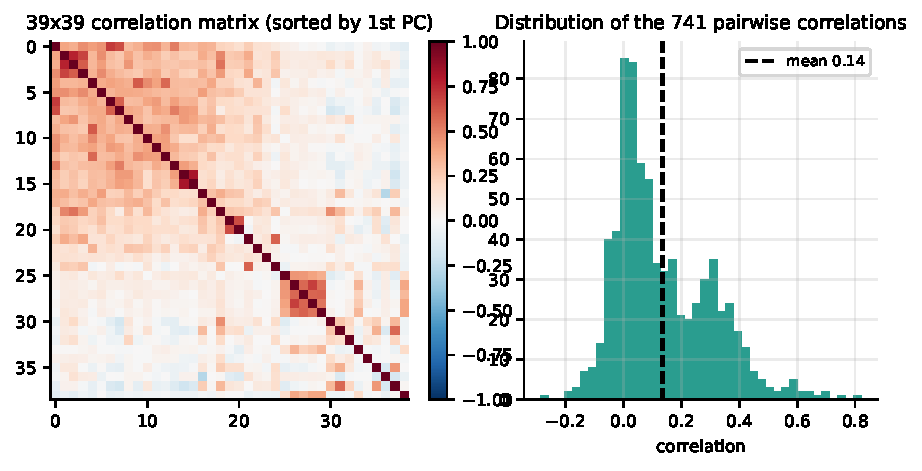
\includegraphics[width=\linewidth]{figures/fig10.pdf}
    \end{column}
    \begin{column}{0.5\textwidth}
      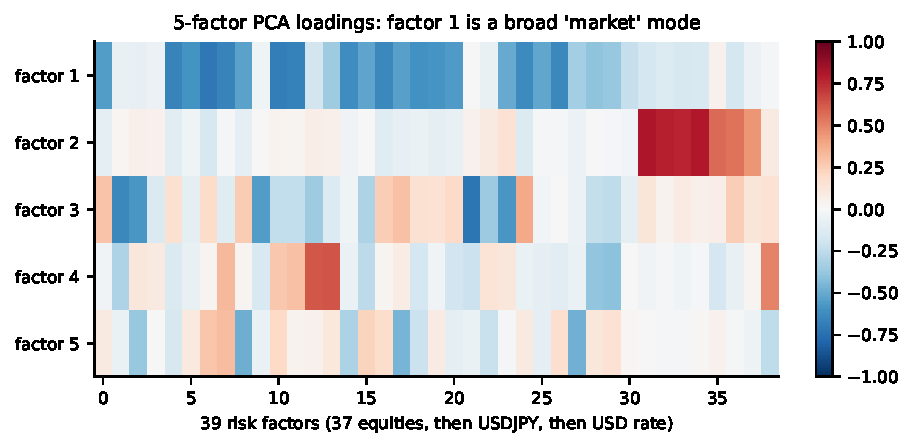
\includegraphics[width=\linewidth]{figures/fig15.pdf}
    \end{column}
  \end{columns}
\end{frame}

\begin{frame}{Appendix: feedback tracker (both rounds)}
  \scriptsize
  \textbf{Earlier meeting} \hfill \textbf{This meeting}
  \begin{columns}[T]
    \begin{column}{0.48\textwidth}
      \begin{enumerate}
        \item Robust stress testing \good
        \item Sensitivities: method, cost, faster alt.\ \good
        \item PCA explainability and speed \good
        \item Final results explanation \good
        \item CVA walkthrough and set-up \good
      \end{enumerate}
    \end{column}
    \begin{column}{0.48\textwidth}
      \begin{enumerate}
        \item[6.] 2008 and more testing periods \good
        \item[7.] LHS to calculate sensitivities \good
        \item[8.] KVA addition \good
        \item[9.] CVA is for sensitivities \good
        \item[10.] DV01 via a Jacobian \good
        \item[11.] Excel parametric vol-bump test \good
      \end{enumerate}
    \end{column}
  \end{columns}
\end{frame}

\begin{frame}{Appendix: simulation grid design}
  \small
  \centering
  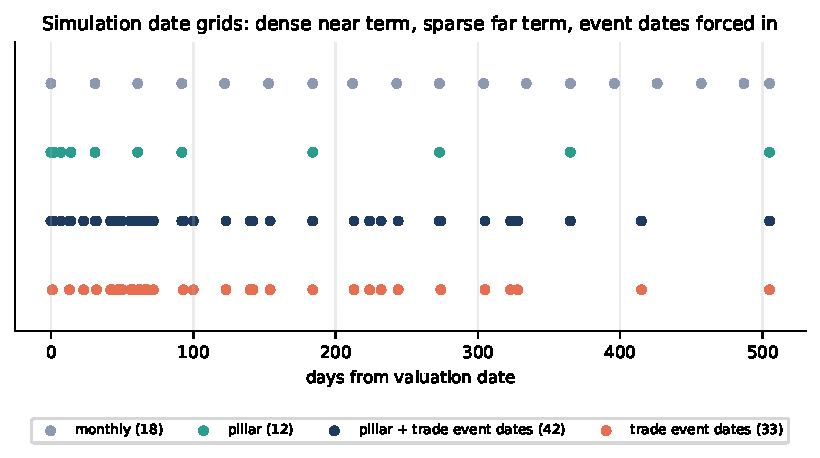
\includegraphics[width=0.75\linewidth]{figures/fig20.pdf}

  \footnotesize The pillar grid (12 dates) plus forced trade-event dates (42 total) is more compact than a plain monthly grid (18) and hits every real cash-flow date exactly.
\end{frame}

\end{document}
